\chapter{Results}
\label{ch:results}
This chapter presents the results of the survey study (chapter \ref{ch:survey}) and the experiments with the value-sensitive rejector (chapter \ref{ch:rejector}).
%
We first present the results of the survey study as the experiments with the value-sensitive rejector depend on the outcomes of the survey study.
%

%
The goal of the survey study was to retrieve the value ratios of TP, TN, FP, FN, and rejected predictions in hate speech detection from the perspective of the social media user.
%
We retrieved the value ratios using the ME scale.
%
We validated the ME scale by conducting a separate survey using a bounded scale of 100 levels, called the 100-level scale.
%
We defined three goals of the experiments with the value-sensitive rejector.
%
First, we want to analyze how the rejector behaves on different models and datasets.
%
Second, we want to find out if rejecting predictions increases the utilities of the ML models in terms of the value of our value-sensitive metric.
%
Finally, we want to compare the value-sensitive metric against machine metrics such as accuracy.
%

%
Section \ref{sec:results-survey-study} covers the results of the complete survey study that we collected after conducting the pilot survey, and section \ref{sec:results-rejector} covers the results of the experiments with the value-sensitive rejector.

\section{Survey study}
\label{sec:results-survey-study}
We collected the responses of all participants to all scenarios for both surveys: one group that uses the ME scale and another that uses the 100-level scale.
%
All participants had to answer two/three questions per scenario, dependent on the choice of the second question.
%

%
The first question asked whether the participant found the content of the social media post hateful or not.
%
Figure \ref{fig:hatefulness} presents the results of the first question by showing the percentages of participants who find the content hateful or not hateful for each scenario.
%
We summed the ME and the 100-level survey responses since this question was the same for both surveys.
%
Most participants agreed with the ground truth label of the social media posts.
%
Please note that according to the ground truth label, REJ1, REJ2, REJ5, and REJ6 are hateful, and REJ3, REJ4, REJ7, and REJ8 are not hateful.
%
So most participants found the posts used in the TP and FN scenarios hateful and those used in TN and FP scenarios not hateful.
%
For the rejection scenarios, most found the posts of REJ1, REJ2, and REJ6 hateful and REJ3, REJ4, and REJ8 not hateful.
%
However, we found three posts where a significant number of participants tended to disagree with the ground truth label (more than or equal to 40\%): FN5, REJ5, and REJ7.
%

%
The second and third questions asked whether the participant agreed/disagreed or was neutral about SocialNet's decision and to what degree.
%
Figure \ref{fig:boxplots} shows the response values to the second and third questions of all scenarios for both scales.
%
Participants generally agreed with the TP and TN scenarios and disagreed with the FP, FN, and rejection scenarios.
%
For both scales, participants disagreed the most with scenarios FN3 and FN7 and agreed the most with scenarios TN3 and TN6.
%
Scenario FN4 was an exception, as some participants agreed with the scenario for both scales.
%

%
The following sections tackle the different parts of the survey analysis: section \ref{sec:results-value-ratios} presents the value ratios required for our value-sensitive rejector, section \ref{sec:results-reliability} presents the reliability analysis, and section \ref{sec:results-validity} the validity analysis.
%
Finally, section \ref{sec:results-demographics} shows the results of the demographic analysis.
%

%
\begin{figure}[t]
    \centering
    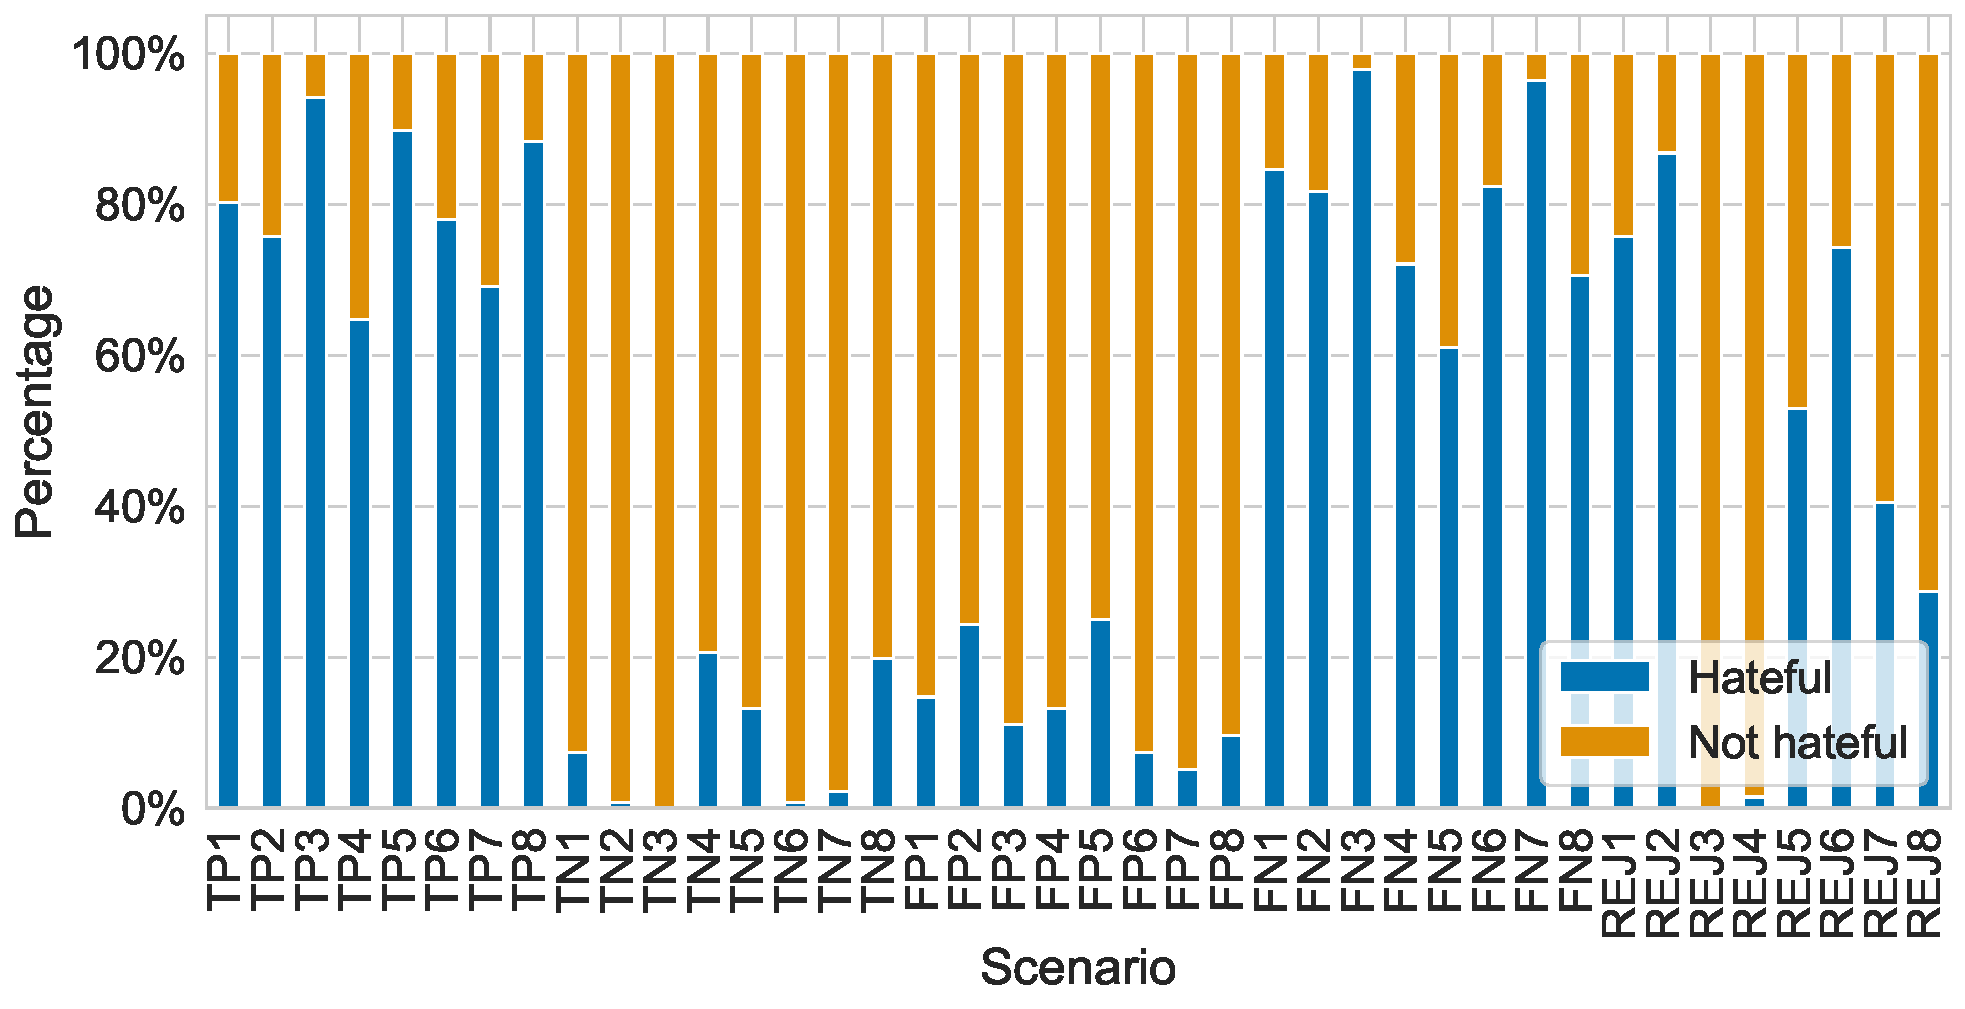
\includegraphics[scale=.4]{Figures/hatefulness.pdf}
    \caption{Stacked bar charts that show the percentages of participants who find the content of the social media post used in the scenarios hateful or not hateful. Each bar is a summation of the responses to both surveys, as this question was the same for both.}
    \label{fig:hatefulness}
\end{figure}
\begin{figure}[h]
    \centering
    \begin{subfigure}[b]{\textwidth}
        \centering
        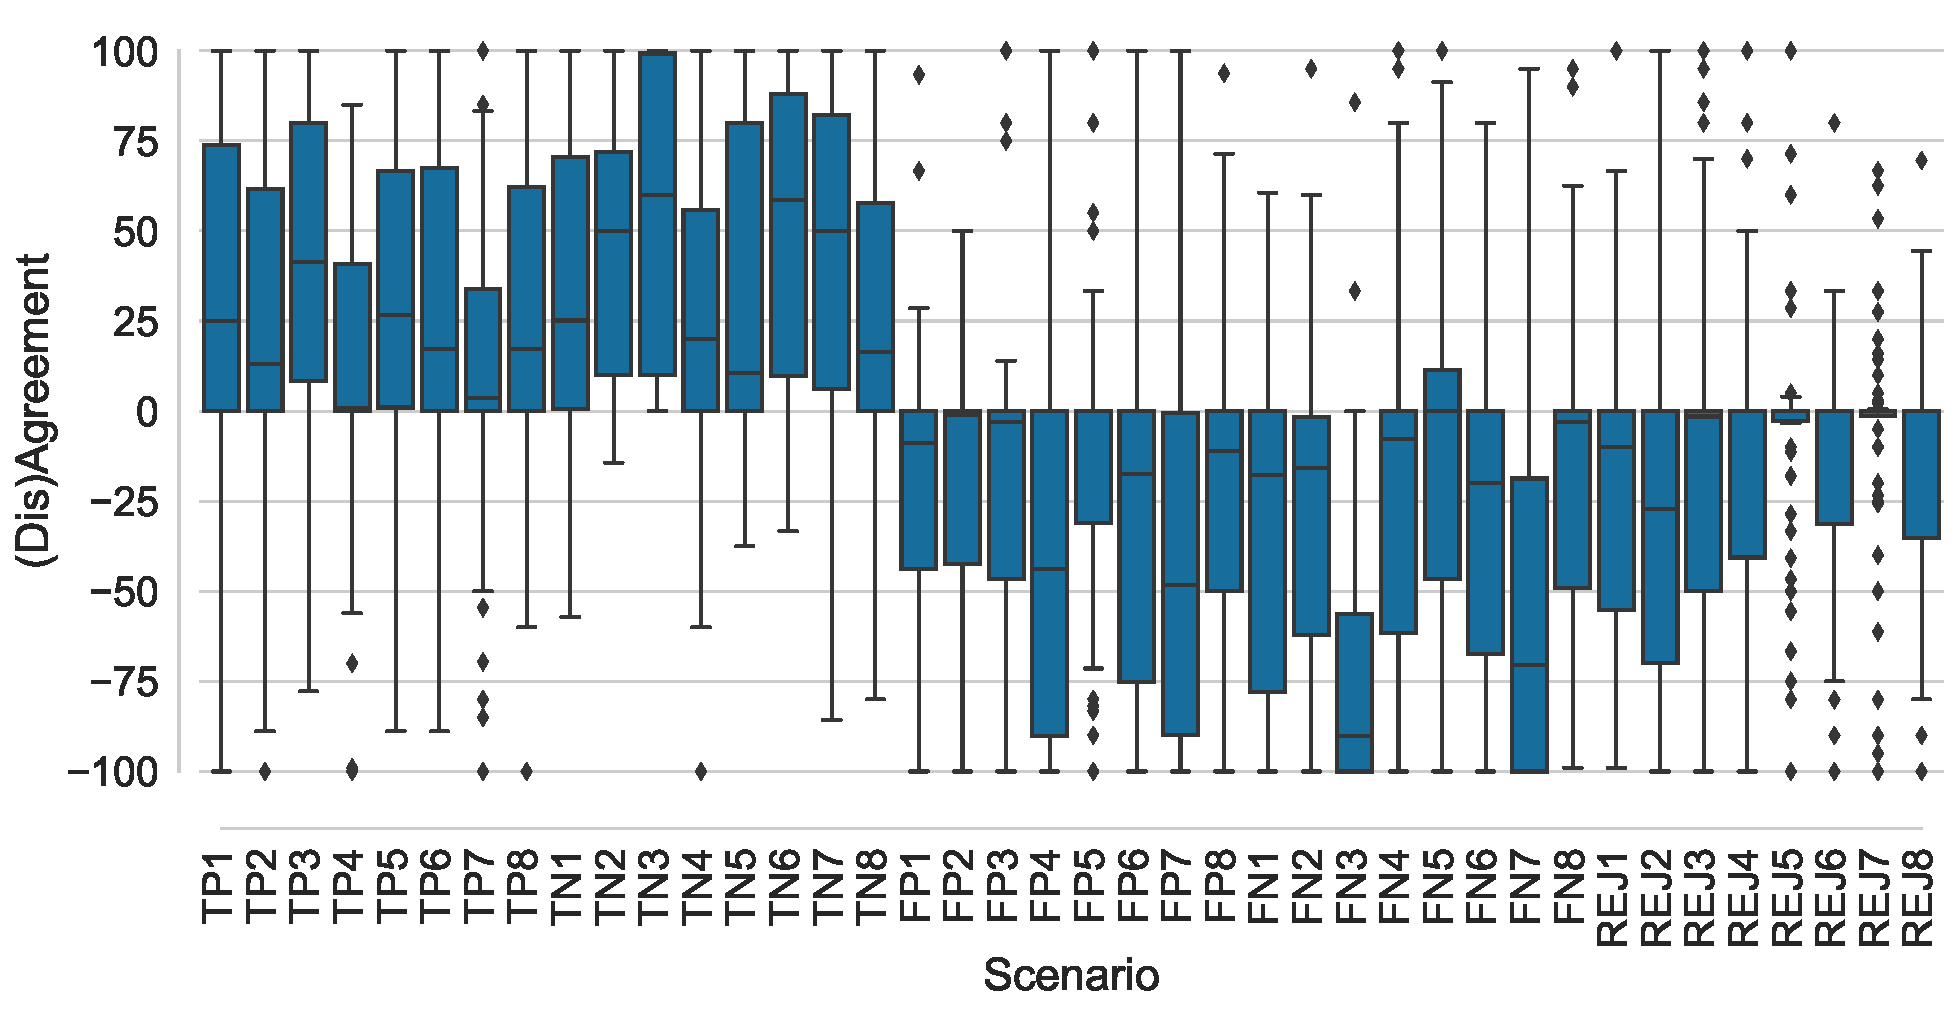
\includegraphics[scale=.4]{Figures/boxplots-ME.pdf}
        \caption{ME scale}
        \label{fig:boxplots-me}
    \end{subfigure}
    \begin{subfigure}[b]{\textwidth}
        \centering
        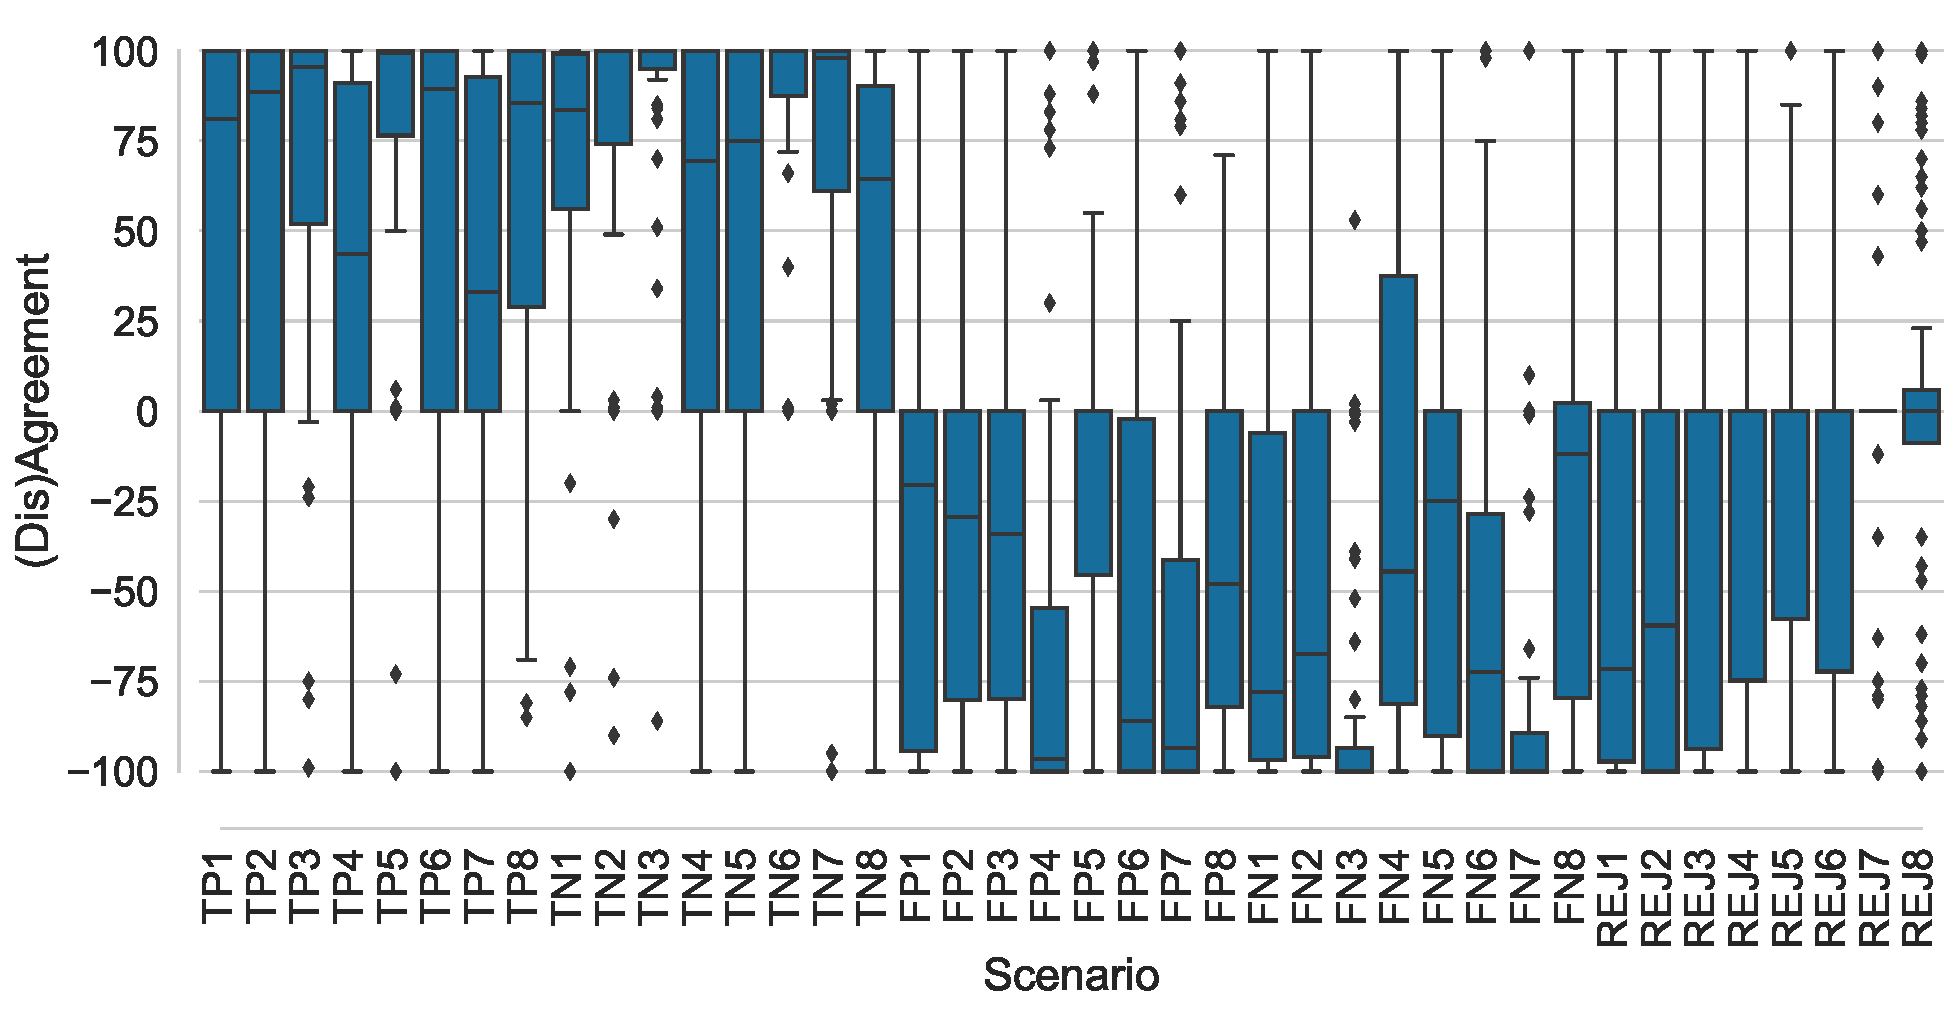
\includegraphics[scale=.4]{Figures/boxplots-100-level.pdf}
        \caption{100-level scale}
        \label{fig:boxplots-100-level}
    \end{subfigure}
    \caption{Boxplots of the responses of all participants to all scenarios for both scales.}
    \label{fig:boxplots}
\end{figure}

\subsection{Value ratios}
\label{sec:results-value-ratios}
We calculated the value ratios following the approach from section \ref{sec:analysis-values}.
%
Table \ref{tab:values-reliability} shows the resulting values ($v$) from the ME and the 100-level surveys.
%
Positive and negative values indicate agreement and disagreement, respectively.
%
For both scales, participants disagreed the most with the FN scenarios and agreed the most with the TN scenarios.
%
The final values of both scales follow the same order: $V_{fn} < V_{fp} < V_{r} < V_{tp} < V_{tn}$.
%
Participants give the highest absolute response values to the TN scenarios.
%
We also observed that participants provided greater absolute response values to the TP and TN scenarios than to the FP and FN scenarios.
%
\begin{table}[t]
    \small
    \centering
    \begin{tabular}{lcccc}
        \toprule
                           & \multicolumn{2}{c}{\textbf{ME}} & \multicolumn{2}{c}{\textbf{100-level}}                                        \\
        \cmidrule(l){2-3} \cmidrule(l){4-5}
                           & $\boldsymbol{\alpha}$           & $\textbf{v}$                           & $\boldsymbol{\alpha}$ & $\textbf{v}$ \\
        \midrule
        \textbf{TP}        & 0.07                            & 18.15                                  & 0.04                  & 77.00        \\
        \textbf{TN}        & 0.10                            & 36.32                                  & 0.11                  & 86.31        \\
        \textbf{FP}        & 0.39                            & -16.69                                 & 0.07                  & -51.00       \\
        \textbf{FN}        & 0.92                            & -28.08                                 & 0.14                  & -62.43       \\
        \textbf{Rejection} & -0.31                           & -4.82                                  & 0.07                  & -16.37       \\
        \midrule
        \textbf{All}       & 0.78                            & ---                                    & 0.44                  & ---          \\
        \bottomrule
    \end{tabular}
    \caption{Krippendorff's alpha ($\alpha$) and the scenario values ($v$) for TP, TN, FP, FN, and rejection scenarios for the ME and 100-level scales.}
    \label{tab:values-reliability}
\end{table}

\subsection{Reliability}
\label{sec:results-reliability}
As explained in section \ref{sec:reliability}, we measured the interrater reliability between the participants using Krippendorff's alpha.
%
Table \ref{tab:values-reliability} shows Krippendorff's alpha ($\alpha$) values for both scales.
%
In the last row of the table, we computed the $\alpha$ values over the responses to all scenarios.
%
The ME scale seemed more reliable than the 100-level scale.
%
According to \citet{krippendorff2004reliability}, the results of the ME scale are reliable, while the results of the 100-level scale are likely to be unreliable.
%

%
We also computed the $\alpha$ values for each group of scenarios of the same type (TP, TN, FP, FN, or rejection).
%
Participants using the ME scale tended to agree with each other on the FP and FN scenarios, while they tended to disagree on the rejection scenarios.
%
For the 100-level scale, we see that participants have low agreement on all scenario types.

\subsection{Validity}
\label{sec:results-validity}
We analyzed the validity of the ME method by performing cross-modality validation between the ME and the 100-level scale (refer to section \ref{sec:analysis-validity}).
%
Figure \ref{fig:correlation} shows the correlation between the ME scale and the 100-level scale.
%
The Shapiro-Wilk test of normality showed that both the median (normalized) ME scores and the median 100-level scores do not follow a normal distribution ($p < 0.05$).
%
We calculated the median because when we look at figure \ref{fig:boxplots}, we can see that the data of both scales are skewed and contain many extreme outliers.
% 
We calculated the Spearman and the Kendall correlation statistics as these are non-parametric and, therefore, do not require the normality assumption.
%
Spearman returned a 0.98 and Kendall a 0.89 correlation between the ME and the 100-level scales ($p < 0.05$), indicating that both scales are highly correlated.

\begin{figure}
    \centering
    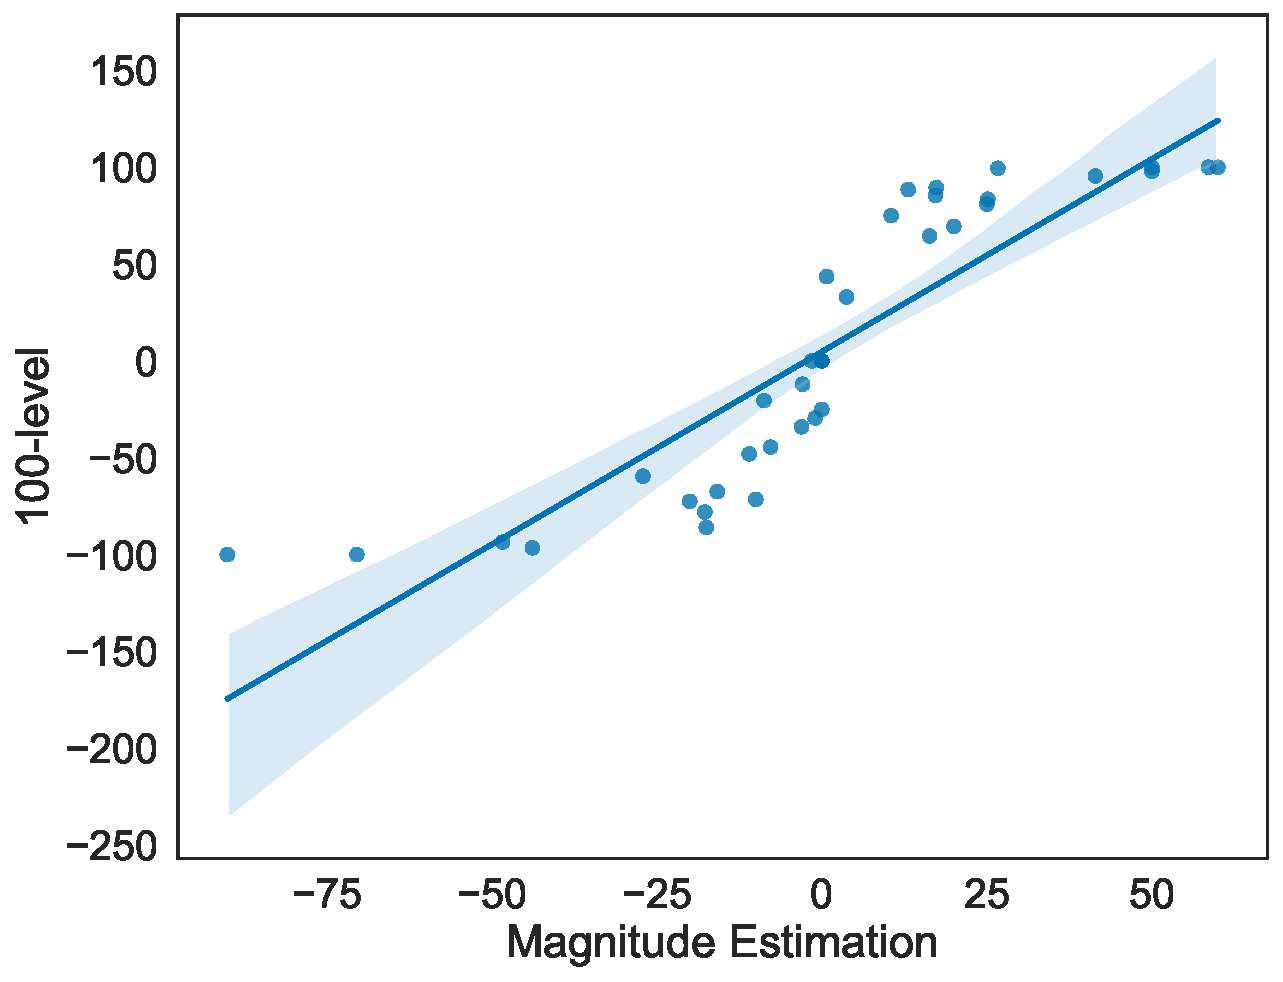
\includegraphics[scale=.4]{Figures/correlation.pdf}
    \caption{Correlation plot between the median normalized magnitude estimates and the median 100-level scores per question.}
    \label{fig:correlation}
\end{figure}

\subsection{Demographics}
\label{sec:results-demographics}
We followed the approach from section \ref{sec:analysis-demographic} to analyze whether statistically significant differences exist between groups with different demographic characteristics.
%
We focused on six features: sex, student, continent, nationality, language, and ethnicity.
%

%
We only used non-parametric statistical tests to analyze the demographic differences for two reasons.
%
First, we found that the assumptions of normality and homogeneity of variances were violated in our dataset when looking at the different groups for all features.
%
Second, we found that for most features, except sex, the sample sizes of the feature groups were not equal.
%
We used Mann-Whitney U to verify a significant difference between the two groups, and we used Kruskal-Wallis for more than two groups.
%

%
Table \ref{tab:results-differences-ind} shows the resulting p values for all scenarios and all features.
%
We found that there are no significant differences between men and women.
%
We found only three scenarios with significant differences for the student and continent features.
%
We found the most significant differences when looking at nationality and language.
%
We observed five scenarios with non-hateful posts and ten scenarios with hateful posts where there is at least one feature with significant differences between the groups.
%
Scenarios FP7 and REJ4 have the most features (4) with significant differences.
%
Scenarios TP6, FN5, and REJ1 have the second most features (2) with significant differences.
%

%
Table \ref{tab:results-differences-grp} shows the p values of the statistical tests for the aggregated scenarios (TP, TN, FP, FN, and rejection) and all features.
%
We aggregated the scores by calculating the mean response value to all scenarios of the same type, e.g. TP, for each participant.
%
Then we applied the statistical tests to the aggregated scores.
%
We found the most significant differences in the aggregated scores of the FP scenarios.
%

%
Finally, we conducted pairwise Mann-Whitney U tests to check if there are any significant differences between pairs of groups for the multi-group features: nationality, language, and ethnicity.
%
Tables \ref{tab:results-pairwise-nationality}, \ref{tab:results-pairwise-language}, and \ref{tab:results-pairwise-ethnicity} present the resulting p values of the pairwise Mann-Whitney U tests for the features of nationality, language, and ethnicity, respectively.
%
We did not find many pairwise significant differences for most of these scenarios and the three features.
%
We found the most pairwise differences (four out of the six pairs) for scenario FN5 and the nationality feature.
%
\begin{table}
    \small
    \centering
    \begin{tabular}{lccc|ccc}
        \toprule
                      & \multicolumn{3}{c}{\textbf{Two groups}} & \multicolumn{3}{c}{\textbf{More than two groups}}                                                                                                                                                                       \\
        \midrule
                      & \multicolumn{1}{c}{\textbf{Sex}}        & \multicolumn{1}{c}{\textbf{Student}}              & \multicolumn{1}{c}{\textbf{Continent}} & \multicolumn{1}{c}{\textbf{Nationality}} & \multicolumn{1}{c}{\textbf{Language}}  & \multicolumn{1}{c}{\textbf{Ethnicity}} \\
        \midrule
        \textbf{TP1}  & 0.506                                   & 0.371                                             & 0.982                                  & 0.095                                    & 0.117                                  & 0.108                                  \\
        \textbf{TP2}  & 0.268                                   & 0.201                                             & 0.387                                  & 0.300                                    & 0.330                                  & 0.464                                  \\
        \textbf{TP3}  & 0.680                                   & 0.276                                             & 0.577                                  & 0.160                                    & \cellcolor[HTML]{EFEFEF}\textbf{0.046} & 0.138                                  \\
        \textbf{TP4}  & 0.756                                   & 0.441                                             & 0.774                                  & 0.137                                    & 0.175                                  & 0.568                                  \\
        \textbf{TP5}  & 0.392                                   & \cellcolor[HTML]{EFEFEF}\textbf{0.011}            & 0.387                                  & 0.152                                    & 0.106                                  & 0.341                                  \\
        \textbf{TP6}  & 0.260                                   & 0.097                                             & 0.682                                  & \cellcolor[HTML]{EFEFEF}\textbf{0.002}   & \cellcolor[HTML]{EFEFEF}\textbf{0.006} & 0.215                                  \\
        \textbf{TP7}  & 0.342                                   & 0.730                                             & 0.059                                  & 0.241                                    & 0.400                                  & 0.238                                  \\
        \textbf{TP8}  & 0.495                                   & \cellcolor[HTML]{EFEFEF}\textbf{0.015}            & 0.246                                  & 0.568                                    & 0.387                                  & 0.190                                  \\
        \textbf{TN1}  & 0.430                                   & 0.480                                             & 0.554                                  & 0.307                                    & 0.260                                  & 0.449                                  \\
        \textbf{TN2}  & 0.567                                   & 0.382                                             & 0.633                                  & 0.595                                    & 0.716                                  & 0.833                                  \\
        \textbf{TN3}  & 0.393                                   & 0.866                                             & 0.766                                  & 0.443                                    & 0.298                                  & 0.432                                  \\
        \textbf{TN4}  & 0.104                                   & 0.171                                             & 0.059                                  & 0.245                                    & 0.251                                  & 0.201                                  \\
        \textbf{TN5}  & 0.290                                   & 0.199                                             & 0.964                                  & 0.304                                    & 0.177                                  & 0.296                                  \\
        \textbf{TN6}  & 0.521                                   & 0.510                                             & 0.608                                  & 0.815                                    & 0.748                                  & 0.600                                  \\
        \textbf{TN7}  & 0.224                                   & 0.878                                             & \cellcolor[HTML]{EFEFEF}\textbf{0.050} & 0.108                                    & 0.223                                  & 0.314                                  \\
        \textbf{TN8}  & 0.191                                   & 0.417                                             & 0.327                                  & 0.168                                    & 0.761                                  & 0.872                                  \\
        \textbf{FP1}  & 0.270                                   & 0.545                                             & 0.065                                  & 0.093                                    & 0.333                                  & 0.174                                  \\
        \textbf{FP2}  & 0.337                                   & 0.114                                             & 0.155                                  & \cellcolor[HTML]{EFEFEF}\textbf{0.008}   & 0.164                                  & 0.195                                  \\
        \textbf{FP3}  & 0.561                                   & 0.509                                             & 0.889                                  & 0.793                                    & 0.725                                  & 0.205                                  \\
        \textbf{FP4}  & 0.278                                   & 0.860                                             & 0.908                                  & 0.267                                    & 0.186                                  & 0.344                                  \\
        \textbf{FP5}  & 0.847                                   & 0.445                                             & 0.220                                  & 0.269                                    & 0.554                                  & 0.194                                  \\
        \textbf{FP6}  & 0.774                                   & 0.266                                             & 0.555                                  & 0.758                                    & 0.409                                  & 0.486                                  \\
        \textbf{FP7}  & 0.391                                   & 0.784                                             & \cellcolor[HTML]{EFEFEF}\textbf{0.015} & \cellcolor[HTML]{EFEFEF}\textbf{0.026}   & \cellcolor[HTML]{EFEFEF}\textbf{0.020} & \cellcolor[HTML]{EFEFEF}\textbf{0.010} \\
        \textbf{FP8}  & 0.624                                   & 0.837                                             & 0.681                                  & 0.544                                    & 0.225                                  & 0.705                                  \\
        \textbf{FN1}  & 0.337                                   & 0.213                                             & 0.317                                  & 0.261                                    & 0.668                                  & 0.558                                  \\
        \textbf{FN2}  & 0.791                                   & 0.928                                             & 0.759                                  & 0.967                                    & 0.974                                  & 0.823                                  \\
        \textbf{FN3}  & 0.990                                   & 0.752                                             & 0.480                                  & 0.504                                    & 0.455                                  & 0.182                                  \\
        \textbf{FN4}  & 0.511                                   & 0.573                                             & 0.450                                  & 0.549                                    & 0.856                                  & 0.965                                  \\
        \textbf{FN5}  & 0.306                                   & 0.467                                             & 0.802                                  & \cellcolor[HTML]{EFEFEF}\textbf{0.001}   & \cellcolor[HTML]{EFEFEF}\textbf{0.009} & 0.349                                  \\
        \textbf{FN6}  & 0.109                                   & 0.113                                             & 0.928                                  & \cellcolor[HTML]{EFEFEF}\textbf{0.012}   & 0.084                                  & 0.436                                  \\
        \textbf{FN7}  & 0.871                                   & 0.677                                             & 0.093                                  & 0.107                                    & \cellcolor[HTML]{EFEFEF}\textbf{0.046} & 0.148                                  \\
        \textbf{FN8}  & 0.776                                   & \cellcolor[HTML]{EFEFEF}\textbf{0.009}            & 0.819                                  & 0.949                                    & 0.363                                  & 0.117                                  \\
        \textbf{REJ1} & 0.799                                   & 0.734                                             & 0.544                                  & \cellcolor[HTML]{EFEFEF}\textbf{0.021}   & \cellcolor[HTML]{EFEFEF}\textbf{0.012} & 0.168                                  \\
        \textbf{REJ2} & 0.644                                   & 0.202                                             & 0.741                                  & 0.295                                    & 0.258                                  & 0.749                                  \\
        \textbf{REJ3} & 0.803                                   & 0.815                                             & 0.108                                  & 0.425                                    & 0.482                                  & 0.133                                  \\
        \textbf{REJ4} & 0.985                                   & 1.000                                             & \cellcolor[HTML]{EFEFEF}\textbf{0.002} & \cellcolor[HTML]{EFEFEF}\textbf{0.014}   & \cellcolor[HTML]{EFEFEF}\textbf{0.036} & \cellcolor[HTML]{EFEFEF}\textbf{0.002} \\
        \textbf{REJ5} & 0.133                                   & 0.994                                             & 0.570                                  & 0.111                                    & \cellcolor[HTML]{EFEFEF}\textbf{0.036} & 0.090                                  \\
        \textbf{REJ6} & 0.244                                   & 0.195                                             & 0.716                                  & 0.061                                    & 0.166                                  & 0.664                                  \\
        \textbf{REJ7} & 0.911                                   & 0.853                                             & 0.942                                  & 0.997                                    & 0.996                                  & \cellcolor[HTML]{EFEFEF}\textbf{0.020} \\
        \textbf{REJ8} & 0.157                                   & 0.167                                             & 0.944                                  & 0.901                                    & 0.741                                  & 0.108                                  \\
        \bottomrule
    \end{tabular}
    \caption{\textbf{Individual}: an overview of the statistical differences between different groups of participants for various demographic characteristics for each scenario in the ME survey. Each cell contains the p value of either the Mann-Whitney U test for two groups or the Kruskal-Wallis test for more than two groups. The grey cells with bold text indicate significant statistical differences between the groups for that feature and scenario type.}
    \label{tab:results-differences-ind}
\end{table}

\section{Value-sensitive rejection}
\label{sec:results-rejector}
We experimented with our value-sensitive rejector following the approach from section \ref{sec:rejector-application}.
%
We produced a set of predictions for each experimental setup, applied our value-sensitive rejector to each setup, and collected the results for analysis.
%

%
We used all three models (LR, DistilBERT, and CNN) to produce predictions for both the \emph{seen} and \emph{unseen} datasets.
%
Therefore, we ended up with six different sets of predictions.
%
Then, for each set of predictions, we created the PDFs for all predictions of the same type (TP, TN, FP, and FN).
%
The PDFs were necessary for calculating the total value of the models with the reject option.
%
Figures \ref{fig:pdfs-seen} and \ref{fig:pdfs-unseen} show all PDFs for the \emph{seen} and \emph{unseen} datasets, respectively.
%
We observed that all three models were more confident in their correct predictions (TP and TN) than their incorrect predictions (FP and FN) for both the \emph{seen} and \emph{unseen} datasets.
%
All three models were also more confident in their correct predictions for the \emph{seen} dataset than the \emph{unseen} dataset.
%
The CNN and LR models have similar PDFs and seem more calibrated since the PDFs of the correct predictions are skewed towards $1.0$.
%
In contrast, the PDFs of the incorrect predictions follow a more uniform distribution.
%
The DistilBERT model is less calibrated than the other two models.
%
We recognize this in the PDFs of the incorrect predictions in figures \ref{fig:pdfs-seen} and \ref{fig:pdfs-unseen} of the DistilBERT model by looking at the large density values around the high confidence values.
%

% Continu
%
We applied the value-sensitive metric from section \ref{sec:value-metric} to the three models and the two datasets using the PDFs and the ME values ($V_{tp}, V_{tn}, V_{fp}, V_{fn}, \text{ and } V_r$) from the survey.
%
Figure \ref{fig:metric-plots-all-values} presents the total value of all models with the reject option ($V(\tau)$) for all possible rejection thresholds ($\tau \in [0.5, 1.0]$) and the ME values from table \ref{tab:values-reliability}.
%
The diamond-shaped markers indicate the optimal rejection threshold ($\tau_O$) for which the model achieves the highest total value ($V(\tau_O)$).
%
Positive $V(\tau)$ values indicate that the model for rejection threshold $\tau$ is valuable, and negative values indicate that the costs of incorrect accepted and rejected predictions exceed the gains of correct accepted and rejected predictions.
%
For all models, we got $\tau_O \approx 0.5$, meaning that all models achieve the highest total value when all predictions are accepted.
%
Figure \ref{fig:metric-plots-all-values} shows that all models' $V(\tau_O)$ values are greater for the \emph{seen} data than for the \emph{unseen} data.
%
The total value of all models decreases for increasing values of the rejection threshold.
%

%
To further examine how $V(\tau)$ behaves when we only consider punishing incorrect predictions instead of rewarding correct predictions, we decided to apply the metric again, setting $V_{tp}$ and $V_{tn}$ equal to zero.
%
The metric's conditions \ref{for:conditions-fp-fn} and \ref{for:conditions-tp-tn} were still satisfied when we did this.
%
Figure \ref{fig:metric-plots-tptn0} presents the total value ($V(\tau)$) again for the updated values $V_{tp}=0$ and $V_{tn}=0$.
%
We found that $\tau_O$ of all models moved towards $1.0$, meaning that rejecting predictions is now more beneficial for the total value of the models.
%
All models achieve the highest $V(\tau)$ value when $\tau \in [0.7, 0.9]$ for \emph{seen} data and when $\tau \in [0.9, 1.0]$ for \emph{unseen data}.
%

%
Table \ref{tab:metric} shows the specific values of $\tau_O$, the accuracies of the accepted predictions, and the rejection rates (fraction of rejected predictions).
%
The first two rows show that the accuracies of all models dropped when we applied the models to \emph{unseen} data.
%
The last two rows (where $V_{tp}=0$ and $V_{tn}=0$) show that we achieved higher accuracies of accepted predictions for increasing optimal rejection thresholds.
%
For all models, we rejected less than 30\% of all predictions for the \emph{seen} data and a large fraction for the \emph{unseen} data.
%
The DistilBERT model achieved the highest accuracies of accepted predictions for all configurations.
%
For the \emph{seen} data, it achieved an accuracy of accepted predictions of $92.6\%$ while rejecting only $25.2\%$ of all predictions.
%
For the \emph{unseen} data, it rejected the least amount of predictions ($92.3\%$) and achieved the highest accuracy of accepted predictions ($88.1\%$).
%
The CNN model performs the worst for all configurations regarding the accuracy of accepted predictions.
%
The model achieved the highest value for the \emph{unseen} data when all predictions were rejected, indicating that it is not valuable to use the model.

%
Table \ref{tab:metric2} compares the results of our value-sensitive metric with machine metrics like accuracy.
%
For all models, it presents the total value for the optimal rejection thresholds ($V(\tau_O)$), the total value when all predictions are accepted ($V(0)$), and the accuracies when all predictions are accepted.
%
First, we compared the accuracy of the original model with $V(0)$, as in both cases, all predictions were accepted.
%
In the first two rows, both the accuracy and $V(0)$ indicate that the DistilBERT model performed the best for both the \emph{seen} and \emph{unseen} datasets.
%
In the last two rows (where $V_{tp}=0$ and $V_{tn}=0$), both metrics indicate that the DistilBERT model performed the best for the \emph{seen} dataset but got different results for the \emph{unseen} dataset.
%
Then, according to the accuracy, the DistilBERT model performed the best, while the CNN model performed the best according to $V(0)$.
%
All $V(0)$ values in the last row show that none of the models is valuable for \emph{unseen} data when we accept all predictions.
%

%
When we look at the $V(\tau_O)$ values in table \ref{tab:metric2}, we see that all models are valuable for the optimal rejection threshold.
%
The DistilBERT model achieved the highest $V(\tau_O)$ values in all configurations except for the \emph{unseen} data with $V_{tp}=0$ and $V_{tn}=0$, as the LR model achieved a higher total value.
%
This result is interesting as we can see from table \ref{tab:metric} that for the DistilBERT model, the accuracy of the accepted predictions is higher, and the rejection rate is lower than for the LR model.
%
Looking at the last row, we can see that all models become valuable when we adopt the optimal rejection threshold.


\begin{figure}
    \centering
    \begin{subfigure}{.49\textwidth}
        \centering
        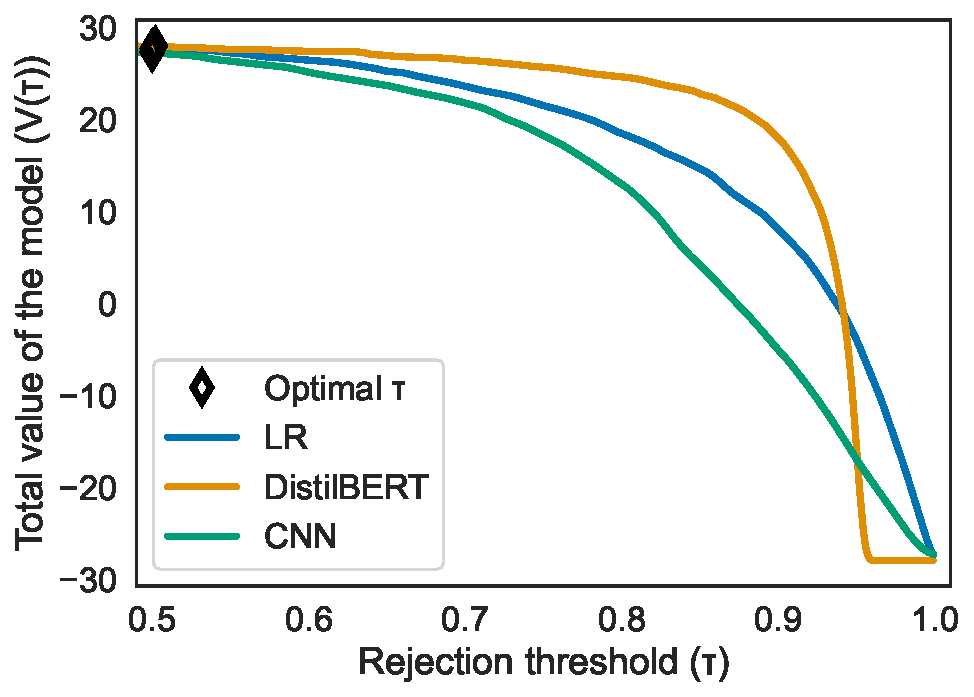
\includegraphics[scale=.4]{Figures/metric-all-values-seen-data.pdf}
        \caption{evaluated on \emph{seen} data}
    \end{subfigure}
    \begin{subfigure}{.49\textwidth}
        \centering
        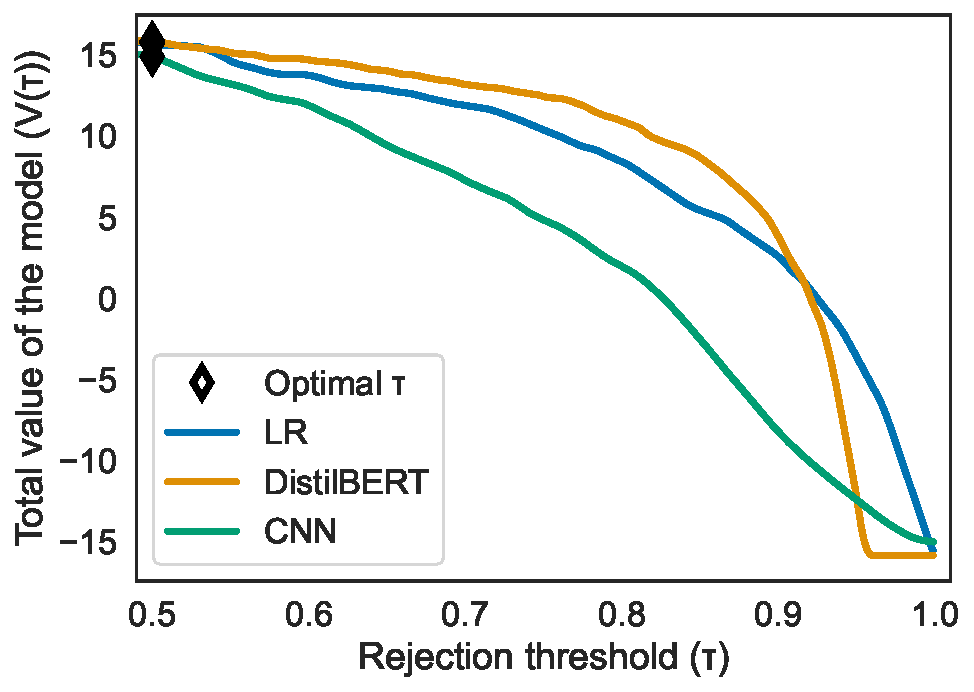
\includegraphics[scale=.4]{Figures/metric-all-values-unseen-data.pdf}
        \caption{evaluated on \emph{unseen} data}
    \end{subfigure}
    \caption{$V(\tau)$ functions of all models with $V_{tp} = 18.15$, $V_{tn} = 36.32$, $V_{fp} = 16.69$, $V_{fn} = 28.08$, $V_r = 4.82$.}
    \label{fig:metric-plots-all-values}
\end{figure}

\begin{figure}
    \centering
    \begin{subfigure}{.49\textwidth}
        \centering
        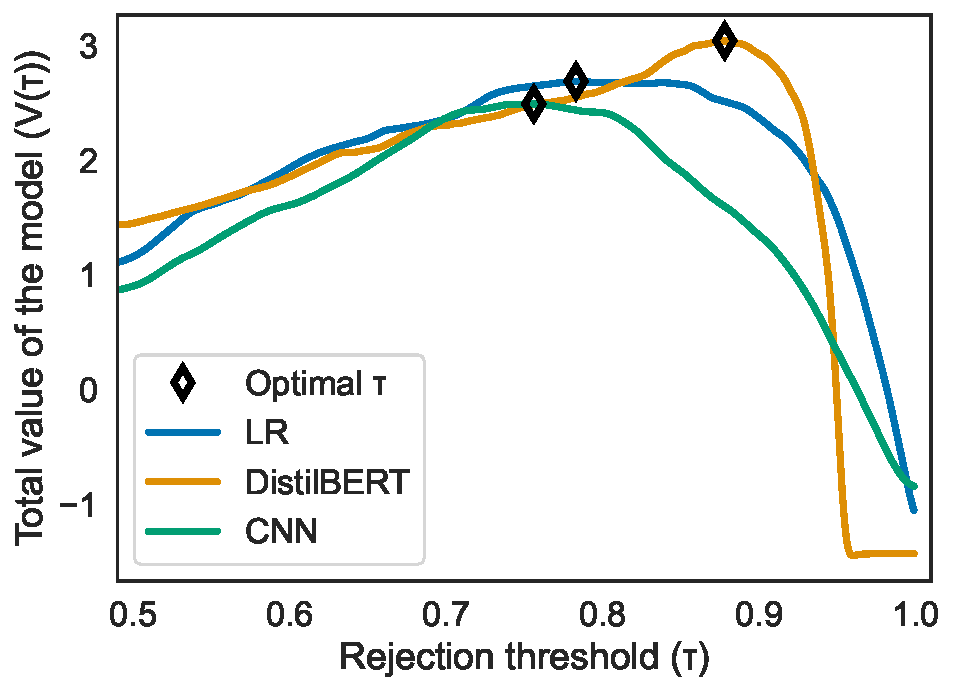
\includegraphics[scale=.4]{Figures/metric-tptn0-seen-data.pdf}
        \caption{evaluated on \emph{seen} data}
    \end{subfigure}
    \begin{subfigure}{.49\textwidth}
        \centering
        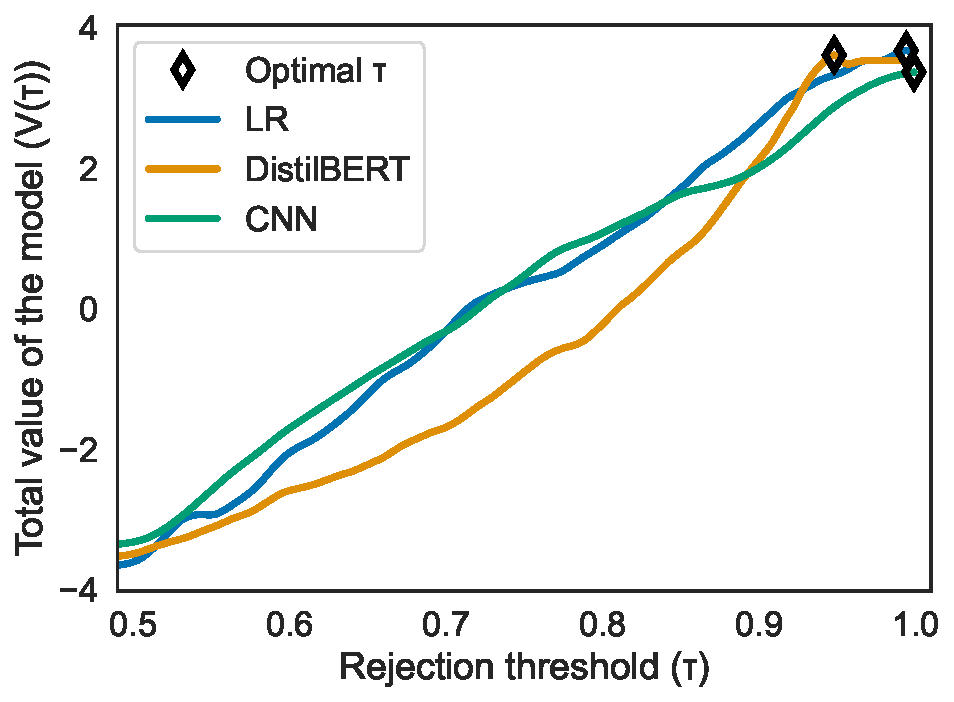
\includegraphics[scale=.4]{Figures/metric-tptn0-unseen-data.pdf}
        \caption{evaluated on \emph{unseen} data}
    \end{subfigure}
    \caption{$V(\tau)$ functions of all models with $V_{tp} = 0.0$, $V_{tn} = 0.0$, $V_{fp} = 16.69$, $V_{fn} = 28.08$, $V_r = 4.82$.}
    \label{fig:metric-plots-tptn0}
\end{figure}

\begin{table}
    \scriptsize
    \centering
    \setlength\tabcolsep{5pt}
    \begin{tabular}{lcccccccccc}
        \toprule
                                                 & \multicolumn{3}{c}{\textbf{LR}} & \multicolumn{3}{c}{\textbf{DistilBERT}} & \multicolumn{3}{c}{\textbf{CNN}}                                                                                                           \\
        \cmidrule(l){2-4} \cmidrule(l){5-7} \cmidrule(l){8-10}
                                                 & $\boldsymbol{\tau_O}$           & \textbf{Acc}                            & \textbf{RR}                      & $\boldsymbol{\tau_O}$ & \textbf{Acc} & \textbf{RR} & $\boldsymbol{\tau_O}$ & \textbf{Acc} & \textbf{RR} \\
        \midrule
        \textbf{Seen data}                       & 0.500                           & 0.847                                   & 0.000                            & 0.502                 & 0.850        & 0.000       & 0.500                 & 0.835        & 0.000       \\
        \textbf{Unseen data}                     & 0.500                           & 0.640                                   & 0.000                            & 0.500                 & 0.640        & 0.000       & 0.500                 & 0.629        & 0.000       \\
        \midrule
        \textbf{Seen data $(V_{tp}=V_{tn}=0)$}   & 0.783                           & 0.910                                   & 0.250                            & 0.878                 & 0.926        & 0.252       & 0.756                 & 0.898        & 0.278       \\
        \textbf{Unseen data $(V_{tp}=V_{tn}=0)$} & 0.994                           & 0.752                                   & 0.958                            & 0.948                 & 0.881        & 0.923       & 0.999                 & -            & 1.0         \\
        \bottomrule
    \end{tabular}
    \caption{The optimal rejection thresholds ($\tau_O$), the accuracy of the accepted predictions (Acc), and the rejection rates (RR) of all models for both datasets.}
    \label{tab:metric}
\end{table}

\begin{table}
    \scriptsize
    \centering
    \setlength\tabcolsep{5pt}
    \begin{tabular}{lcccccccccc}
        \toprule
                                                 & \multicolumn{3}{c}{\textbf{LR}} & \multicolumn{3}{c}{\textbf{DistilBERT}} & \multicolumn{3}{c}{\textbf{CNN}}                                                                                                                                 \\
        \cmidrule(l){2-4} \cmidrule(l){5-7} \cmidrule(l){8-10}
                                                 & $\boldsymbol{V(\tau_O)}$        & $\boldsymbol{V(0)}$                     & \textbf{Acc}                     & $\boldsymbol{V(\tau_O)}$ & $\boldsymbol{V(0)}$ & \textbf{Acc} & $\boldsymbol{V(\tau_O)}$ & $\boldsymbol{V(0)}$ & \textbf{Acc} \\
        \midrule
        \textbf{Seen data}                       & 27.707                          & 27.707                                  & 0.847                            & 28.001                   & 27.996              & 0.850        & 27.291                   & 27.291              & 0.835        \\
        \textbf{Unseen data}                     & 15.689                          & 15.689                                  & 0.640                            & 15.823                   & 15.823              & 0.640        & 14.868                   & 14.868              & 0.629        \\
        \midrule
        \textbf{Seen data $(V_{tp}=V_{tn}=0)$}   & 2.688                           & 1.158                                   & 0.847                            & 3.041                    & 1.448               & 0.850        & 2.490                    & 0.901               & 0.835        \\
        \textbf{Unseen data $(V_{tp}=V_{tn}=0)$} & 3.668                           & -3.605                                  & 0.640                            & 3.606                    & -3.489              & 0.640        & 3.365                    & -3.322              & 0.629        \\
        \bottomrule
    \end{tabular}
    \caption{The maximum total values of the models for the optimal rejection threshold ($V(\tau_O)$), the total value of the models when all predictions are accepted ($V(0)$), and the accuracies (Acc) of all models.}
    \label{tab:metric2}
\end{table}